\subsection{Fundamentals of Photovoltaik systems}

A Photovoltaic systems transduces solar radiation into electricity. The efficiency of a system depends on the properties of the used photovoltaic cells. Wagner (2010) \citen{Wagner2010} \\

\begin{figure}[hbt!]
\centering
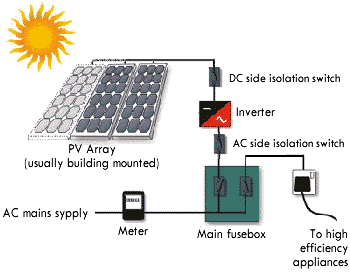
\includegraphics[width=0.7\textwidth]{phase2/group2/figure/pv-system-configuration.png}
\caption{Architecture of Photovaltaic system}
\label{fig:PV_system}
\end{figure}

The nominal power of a cell is given in Watt and often denoted as \(W_p\) (Watt Peak). It is acquired under standard test condition (STC an international standard) from the manufacturer of the photovoltaic cell. STC means, that the cell temperatur is \(25^\circ C\) and the irradiance is 1000 \(W/m^2\). The nominal power can be used to compare the power of photovoltiac cells of different manufactures. 
\\
The efficiency is given by the ratio between the produced energy and the energy radiated to the cell. It depends on the temperature of the photovoltaic cells. With increasing temperature the efficiency decreases. Often only one efficiency coefficient, including the efficiency of the power inverter, cable and accumulator, is given by the manufacturers.
\\
In addition a performance ratio is given most times. It is the ratio of the actual and the desired gain of the photovoltaic cell. It depends not only on the cell itself but also on the weather conditions, respectivly on the location. The desired gain is the efficiency of the installation under STC, assuming that the efficiency of the power inverter is \(100\%\). For a thin-layerd slicon cell, which is most common, the Performance ratio (PR) is \(84\% \) for Germany.
Wagner (2010)

